\documentclass{bioinfo}
\copyrightyear{2012}
\pubyear{2012}

\begin{document}

\title[Scythe]{Supplementary Materials}
\author[Buffalo \textit{et~al}]{Vince Buffalo\,$^{1}$, Joseph Fass\,$^{1}$ and Dawei Lin\,$^1$}
\address{$^{1}$Bioinformatics Core, UC Davis Genome Center}


\history{}

\editor{}

\maketitle

\section{Read Base Quality}

Using the Bioconductor package \texttt{qrqc} (\citealp{qrqc}), we can
get a sense of quality variability by base and the 3'-end
deterioration (see Fig. \ref{fig:01}).


\begin{figure}[!tpb]%figure1
\centerline{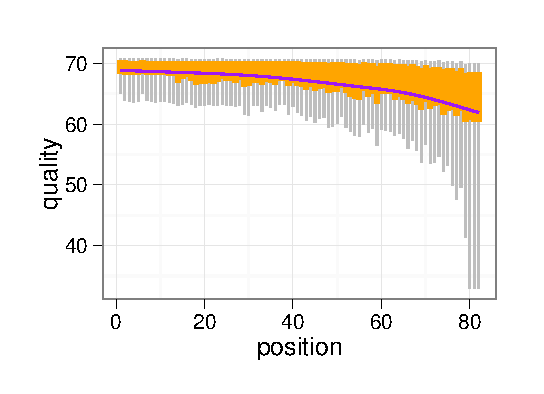
\includegraphics{graphics/qrqc.eps}}
\caption{\texttt{qrqc} quality plot showing base-level quality
  variation and 3'-end deterioration. The grey lines indicate the 10\%
  and 90\% quantile range, the orange lines the interquartile range,
  and the purple line a lowess curve.}
\label{fig:01}
\end{figure}


\section{Time Complexity Calculation}

For an adapter with length $l_a$, there are 
$\sum_{k=1}^{l_a} k = \frac{l_a (l_a + 1)}{2}$ alignments to the 3'-end of reads (assuming no
minimum match). Thus for $R$ reads, the time complexity is:

$$ R \frac{l_a(l_a + 1)}{2} = R \frac{l_a^2 + l_a}{2} = O(l_a^2 R)$$

\section{Quality Trimming}

Since Scythe incorporates base-level quality data in the decision to
trim a suspected contaminant, it is recommended that Scythe be run
\emph{before} a quality trimmer.

We have used Scythe in conjunction with the 5'- and 3'-end sliding
window quality trimmer Sickle (written by Nikhil Joshi and Vince
Buffalo) with positive results. Sickle is available on Github at
\href{http://github.com/najoshi/sickle}{http://github.com/najoshi/sickle}.

\section{Calculation of True Positives, False Positives, and
  Incorrectly Trimmed Reads}

To assess incorrect trimming rates, we calculate the number of reads
that were contaminated and trimmed, and where the length of the
contaminant doesn't match the trimmed length.

\section{Specifying Scythe's Prior}

The prior doesn't need to be estimated increadibly well; one technique
that works well is to view the FASTQ file in the Unix command line
tool \texttt{less} and search for the 3'-end bases of the adapter
contaminant. The number of results on a page of less output divided by
the number of FASTQ entries on that page works well as an initial
guess for the prior.



\bibliographystyle{natbib}
\bibliography{references}


\end{document}
